\documentclass{lab}

\renewcommand{\AA}{\ensuremath{\mathring{A}}}

\begin{document}

\labtitle{4.3.2}{Дифракция на ультразвуковой волне в жидкости}{21~февраля~2019~г.}{28~февраля~2019~г.}

\section*{Постановка эксперимента}

\begin{quote}
	\textbf{{\normalsize Цель работы: }}
	изучить дифракцию света на синусоидальной акустической
	решетке и фазовую решетку методом темного поля.
\end{quote}

\begin{quote}
	\textbf{{\normalsize Оборудование: }}
	оптическая скамья, осветитель, два
	длиннофокусных объектива, кювета с жидкостью, кварцевый излучатель с
	микрометрическим винтом, генератор ультразвуковой частоты, линза,
	вертикальная нить на рейтере, микроскоп.
\end{quote}

\subsection*{Схема установки}

\begin{figure}[H]
	\centering
	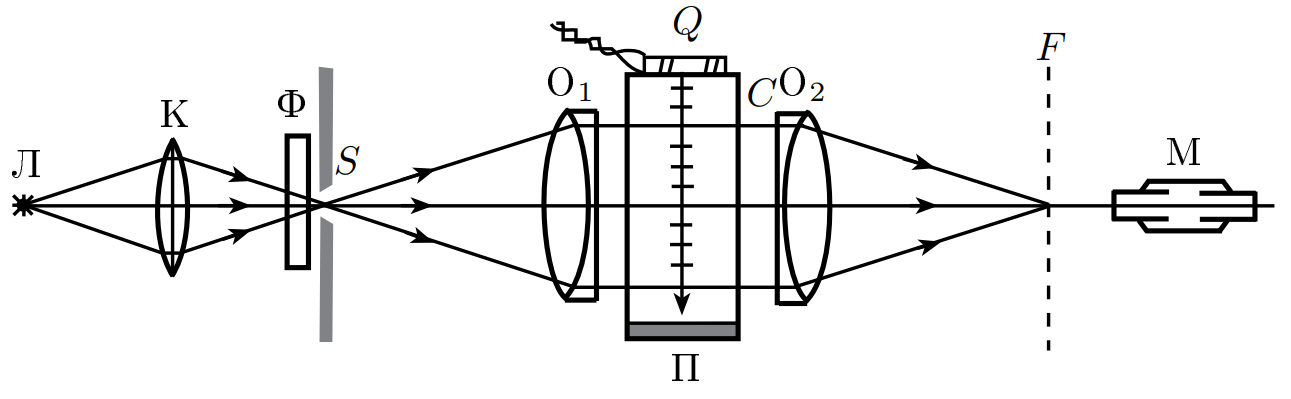
\includegraphics[width = \textwidth]{scheme}
	\caption{Схема установки для наблюдения дифракции на акустической решетке}
	\label{scheme}
\end{figure}

\subsection*{Теоретическая часть}

Изменение показателя преломления жидкости (фаза световых колебаний):
\begin{equation}
n = n_0 (1 + a \cdot \cos (Kx))
\end{equation}
где $ K = 2 \pi / \Lambda $ -- волновое число для УЗ-волны.\\
Условие чистой фазовой решетки:
\begin{equation}
a \ll \left( \frac{\Lambda}{L} \right)^2
\end{equation}
где $ L $ -- толщина слоя жидкости.\\
Условие максимумов в дифракционной картине:
\begin{equation}
\Lambda \cdot \sin (\psi_m) = m \lambda
\end{equation}
Расстояние от центрального до $ m $-го максимума:
\begin{equation}
l_m = \frac{m f \lambda}{\Lambda}
\end{equation}
Скорость распространения волны при известной частоте кварцевого излучателя:
\begin{equation}
v = \Lambda \nu
\end{equation}

\newpage

\subsection*{Выполнение работы}

\subsubsection*{Определение скорости УЗ-волны по дифракционной картине}

Красный цвет:
\begin{equation}
\begin{aligned}
&\lambda = (6400 \pm 200)~\AA\\
&F = 30~см
\end{aligned}
\end{equation}

\begin{enumerate}
\item
Оценим по порядку величины длину УЗ-волны как удвоенное расстояние между максимумами дифракционных картин, наблюдаемых при помощи микроскопа.
\begin{equation}
\nu = 1.08~МГц ~~~~~ \lambda / 2 = 1.43 \cdot 10^{-3}~м
\end{equation}
Тогда $ v = 1544~м/с $ -- скорость УЗ-волны.

\item
Измерим положения $ x_m $ дифракционных максимумов с помощью микрометра для нескольких частот. Данные занесем в таблицу.
\begin{table}[H]
	\centering
	\begin{tabular}{|c|cccc|}
		\hline
		$ \nu,~КГц $ & 1008 & 1014 & 1060 & 1076 \\ \hline
		$ m $        & \multicolumn{4}{c|}{$ x_m $}\\ \hline
		-4 & 24  & 64  & 35  & 35  \\
		-3 & 56  & 97  & 69  & 69  \\
		-2 & 91  & 130 & 102 & 104 \\
		-1 & 123 & 163 & 137 & 138 \\
		0  & 156 & 196 & 172 & 171 \\
		1  & 191 & 229 & 205 & 206 \\
		2  & 222 & 262 & 238 & 240 \\
		3  & 254 & 295 & 273 & 272 \\
		4  & 288 & 328 & 308 & 307 \\ \hline
	\end{tabular}
	\caption{Положения максимумов дифракционных картин для разных частот}
	\label{tab 1}
\end{table}

\item
Построим графики зависимостей из таблицы \ref{tab 1}.
\begin{figure}[H]
\centering
\begin{tikzpicture}
	\begin{axis}[
		width=0.55\textwidth,
		grid=major,
		xlabel = m,
		ylabel = $ x_m \text{, дел} $,
		ymin=0
	]
	\addplot[
		color=red,
		mark=*,
		error bars/.cd,
		x dir=both,
		x explicit,
		y dir=both,
		y explicit,
	] 
	coordinates {
		(-4,24)		+- (0,10)
		(-3,56)		+- (0,10)
		(-2,91)		+- (0,10)
		(-1,123)	+- (0,10)
		(0,156)		+- (0,10)
		(1,191)		+- (0,10)
		(2,222)		+- (0,10)
		(3,254)		+- (0,10)
		(4,288)		+- (0,10)
	};
	\end{axis}
\end{tikzpicture}
\caption{Зависимость $ x_m = f(m) $ при $ \nu = 1008~КГц $}
\label{1}
\end{figure}

\begin{figure}[H]
	\centering
	\begin{tikzpicture}
	\begin{axis}[
	width=0.8\textwidth,
	grid=major,
	xlabel = m,
	ylabel = $ x_m \text{, дел} $,
	ymin=0
	]
	\addplot[
	color=red,
	mark=*,
	error bars/.cd,
	x dir=both,
	x explicit,
	y dir=both,
	y explicit
	] 
	coordinates {
		(-4, 64)		+- (0,10)
		(-3, 97)		+- (0,10)
		(-2, 130)		+- (0,10)
		(-1, 163)		+- (0,10)
		(0,  196)		+- (0,10)
		(1,  229)		+- (0,10)
		(2,  262)		+- (0,10)
		(3,  295)		+- (0,10)
		(4,  328)		+- (0,10)
	};
	\end{axis}
	\end{tikzpicture}
	\caption{Зависимость $ x_m = f(m) $ при $ \nu = 1014~КГц $}
	\label{2}
\end{figure}

\begin{figure}[H]
	\centering
	\begin{tikzpicture}
	\begin{axis}[
	width=0.8\textwidth,
	grid=major,
	xlabel = m,
	ylabel = $ x_m \text{, дел} $,
	ymin=0
	]
	\addplot[
	color=red,
	mark=*,
	error bars/.cd,
	x dir=both,
	x explicit,
	y dir=both,
	y explicit
	] 
	coordinates {
		(-4, 35)		+- (0,10)
		(-3, 69)		+- (0,10)
		(-2, 102)		+- (0,10)
		(-1, 137)		+- (0,10)
		(0,  172)		+- (0,10)
		(1,  205)		+- (0,10)
		(2,  238)		+- (0,10)
		(3,  273)		+- (0,10)
		(4,  308)		+- (0,10)
	};
	\end{axis}
	\end{tikzpicture}
	\caption{Зависимость $ x_m = f(m) $ при $ \nu = 1060~КГц $}
	\label{3}
\end{figure}

\begin{figure}[H]
	\centering
	\begin{tikzpicture}
	\begin{axis}[
	width=0.65\textwidth,
	grid=major,
	xlabel = m,
	ylabel = $ x_m \text{, дел} $,
	ymin=0
	]
	\addplot[
%	only marks,
	color=red,
	mark=*,
	error bars/.cd,
	x dir=both,
	x explicit,
	y dir=both,
	y explicit
	] 
	coordinates {
		(-4, 35)		+- (0,10)
		(-3, 69)		+- (0,10)
		(-2, 104)		+- (0,10)
		(-1, 138)		+- (0,10)
		(0,  171)		+- (0,10)
		(1,  206)		+- (0,10)
		(2,  240)		+- (0,10)
		(3,  272)		+- (0,10)
		(4,  307)		+- (0,10)
	};
	\end{axis}
	\end{tikzpicture}
	\caption{Зависимость $ x_m = f(m) $ при $ \nu = 1076~КГц $}
	\label{4}
\end{figure}

\item
Из графиков (рис. \ref{1}-\ref{4}) определим наклон, а по нему длину и скорость УЗ-волны в воде. Результаты представим в таблице:
\begin{table}[H]
	\centering
	\begin{tabular}{|c|ccc|}
		\hline
		$ \nu,~МГц $ & $ \Delta x,~дел $ & $ \Lambda,~мм $ & $ v,~м/с $ \\ \hline
		1.008 & 33.00 & 1.456 & 1466 \\
		1.014 & 33.00 & 1.454 & 1474 \\
		1.060 & 34.07 & 1.411 & 1496 \\
		1.076 & 33.93 & 1.391 & 1497 \\ \hline
	\end{tabular}
	\caption{Скорость УЗ-волны в жидкости}
	\label{tab 2}
\end{table}

Усредняя полученные результаты из таблицы \ref{tab 2}:
\begin{equation}
v = (1484 \pm 50)м/с, ~~~~~ \varepsilon = 3.4\%
\end{equation}

\end{enumerate}

\subsubsection*{Определение скорости звука методом темного поля}

\begin{enumerate}
\item
Снимем зависимость расстояния и количества темных полос от частоты УЗ-волны.
\begin{table}[H]
	\centering
	\begin{tabular}{|c|ccc|}
		\hline
		$ \nu,~МГц $ & $ \Delta l,~дел $ & $ N,~шт $ & $ \Lambda,~мм $ \\ \hline
		1.1028 & 330 & 4  & 1.395 \\
		1.1659 & 310 & 14 & 1.310 \\
		1.2265 & 340 & 16 & 1.258 \\
		1.2749 & 327 & 16 & 1.209 \\ \hline
	\end{tabular}
	\caption{Темные полосы УЗ-волны в жидкости}
	\label{tab 3}
\end{table}

\item
Построим зависимость $ \Lambda = f(1 / \nu) $ и по нему найдем скорость УЗ-волны в воде (данные из таблицы \ref{tab 3}):
\begin{figure}[H]
	\centering
	\begin{tikzpicture}
	
	\pgfplotstableread{
		X	Y		x-err	y-err
		907	1.395	007		0.03
		858	1.310	007		0.03 
		815	1.258	007		0.02
		784	1.209	007		0.02
	}{\mytable}
	
	\begin{axis}[
		width=0.8\textwidth,
		grid=major,
		xlabel = $ 1 / \nu \text{,} ~ 10^3 ~ \text{c} $,
		ylabel = $ \Lambda \text{, мм} $
	]
	
	\addplot[
		only marks,
		color=red,
		mark=*,
		error bars/.cd,
		x dir=both,
		x explicit,
		y dir=both,
		y explicit
	]
	table[
		x error=x-err,
		y error=y-err
	] {\mytable};

	\addplot[
		mark=none,
		color=red
	]
	table[
		y={create col/linear regression={y=Y}}
	] % compute a linear regression from the
	{\mytable};

	\end{axis}
	\end{tikzpicture}
	\caption{Зависимость $ \Lambda = f(1 / \nu) $}
	\label{5}
\end{figure}

\item
Из графика (рис. \ref{5}) получаем:
\begin{equation}
v = (1480 \pm 60)~м/с, ~~~~~ \varepsilon = 4\%
\end{equation}

\end{enumerate}

\subsection*{Итоги}
Была изучена дифракция света на синусоидальной решетке вертикальной щели.\\

Была вычислена скорость УЗ-волны в воде тремя способами:
\begin{equation}
\begin{aligned}
1. ~~~ &v = 1544~м/с \\
2. ~~~ &v = (1484 \pm 50)~м/с, ~~~~~ \varepsilon = 3.4 \% \\
3. ~~~ &v = (1480 \pm 60)~м/с, ~~~~~ \varepsilon = 4   \% \\
&v_{табл} = 1488~м/с~при~T = 22^{\circ}С
\end{aligned}
\end{equation}

\end{document}